\documentclass[twoside]{book}

% Packages required by doxygen
\usepackage{fixltx2e}
\usepackage{calc}
\usepackage{doxygen}
\usepackage[export]{adjustbox} % also loads graphicx
\usepackage{graphicx}
\usepackage[utf8]{inputenc}
\usepackage{makeidx}
\usepackage{multicol}
\usepackage{multirow}
\PassOptionsToPackage{warn}{textcomp}
\usepackage{textcomp}
\usepackage[nointegrals]{wasysym}
\usepackage[table]{xcolor}

% Font selection
\usepackage[T1]{fontenc}
\usepackage[scaled=.90]{helvet}
\usepackage{courier}
\usepackage{amssymb}
\usepackage{sectsty}
\renewcommand{\familydefault}{\sfdefault}
\allsectionsfont{%
  \fontseries{bc}\selectfont%
  \color{darkgray}%
}
\renewcommand{\DoxyLabelFont}{%
  \fontseries{bc}\selectfont%
  \color{darkgray}%
}
\newcommand{\+}{\discretionary{\mbox{\scriptsize$\hookleftarrow$}}{}{}}

% Page & text layout
\usepackage{geometry}
\geometry{%
  a4paper,%
  top=2.5cm,%
  bottom=2.5cm,%
  left=2.5cm,%
  right=2.5cm%
}
\tolerance=750
\hfuzz=15pt
\hbadness=750
\setlength{\emergencystretch}{15pt}
\setlength{\parindent}{0cm}
\setlength{\parskip}{3ex plus 2ex minus 2ex}
\makeatletter
\renewcommand{\paragraph}{%
  \@startsection{paragraph}{4}{0ex}{-1.0ex}{1.0ex}{%
    \normalfont\normalsize\bfseries\SS@parafont%
  }%
}
\renewcommand{\subparagraph}{%
  \@startsection{subparagraph}{5}{0ex}{-1.0ex}{1.0ex}{%
    \normalfont\normalsize\bfseries\SS@subparafont%
  }%
}
\makeatother

% Headers & footers
\usepackage{fancyhdr}
\pagestyle{fancyplain}
\fancyhead[LE]{\fancyplain{}{\bfseries\thepage}}
\fancyhead[CE]{\fancyplain{}{}}
\fancyhead[RE]{\fancyplain{}{\bfseries\leftmark}}
\fancyhead[LO]{\fancyplain{}{\bfseries\rightmark}}
\fancyhead[CO]{\fancyplain{}{}}
\fancyhead[RO]{\fancyplain{}{\bfseries\thepage}}
\fancyfoot[LE]{\fancyplain{}{}}
\fancyfoot[CE]{\fancyplain{}{}}
\fancyfoot[RE]{\fancyplain{}{\bfseries\scriptsize Generated by Doxygen }}
\fancyfoot[LO]{\fancyplain{}{\bfseries\scriptsize Generated by Doxygen }}
\fancyfoot[CO]{\fancyplain{}{}}
\fancyfoot[RO]{\fancyplain{}{}}
\renewcommand{\footrulewidth}{0.4pt}
\renewcommand{\chaptermark}[1]{%
  \markboth{#1}{}%
}
\renewcommand{\sectionmark}[1]{%
  \markright{\thesection\ #1}%
}

% Indices & bibliography
\usepackage{natbib}
\usepackage[titles]{tocloft}
\setcounter{tocdepth}{3}
\setcounter{secnumdepth}{5}
\makeindex

% Hyperlinks (required, but should be loaded last)
\usepackage{ifpdf}
\ifpdf
  \usepackage[pdftex,pagebackref=true]{hyperref}
\else
  \usepackage[ps2pdf,pagebackref=true]{hyperref}
\fi
\hypersetup{%
  colorlinks=true,%
  linkcolor=blue,%
  citecolor=blue,%
  unicode%
}

% Custom commands
\newcommand{\clearemptydoublepage}{%
  \newpage{\pagestyle{empty}\cleardoublepage}%
}

\usepackage{caption}
\captionsetup{labelsep=space,justification=centering,font={bf},singlelinecheck=off,skip=4pt,position=top}

%===== C O N T E N T S =====

\begin{document}

% Titlepage & ToC
\hypersetup{pageanchor=false,
             bookmarksnumbered=true,
             pdfencoding=unicode
            }
\pagenumbering{alph}
\begin{titlepage}
\vspace*{7cm}
\begin{center}%
{\Large Terprescue Module \\[1ex]\large 1.\+0 }\\
\vspace*{1cm}
{\large Generated by Doxygen 1.8.13}\\
\end{center}
\end{titlepage}
\clearemptydoublepage
\pagenumbering{roman}
\tableofcontents
\clearemptydoublepage
\pagenumbering{arabic}
\hypersetup{pageanchor=true}

%--- Begin generated contents ---
\chapter{Class Index}
\section{Class List}
Here are the classes, structs, unions and interfaces with brief descriptions\+:\begin{DoxyCompactList}
\item\contentsline{section}{\hyperlink{classExplorer}{Explorer} \\*This class contains methods to help the robot navigate and explore the environment }{\pageref{classExplorer}}{}
\item\contentsline{section}{\hyperlink{classLocalizer}{Localizer} \\*The class has can use input data of lidar, camera and also robot\textquotesingle{}s frame to recognize tags and get tags\textquotesingle{} location and ID }{\pageref{classLocalizer}}{}
\item\contentsline{section}{\hyperlink{classTerpRescue}{Terp\+Rescue} \\*The class has functions to subscribe all sensor data and also calculate tag location and display map in R\+Viz }{\pageref{classTerpRescue}}{}
\end{DoxyCompactList}

\chapter{File Index}
\section{File List}
Here is a list of all documented files with brief descriptions\+:\begin{DoxyCompactList}
\item\contentsline{section}{include/\hyperlink{explorer_8hpp}{explorer.\+hpp} \\*This file contains delarations for the \hyperlink{classExplorer}{Explorer} class, which contains methods to help the robot navigate and explore the environment }{\pageref{explorer_8hpp}}{}
\item\contentsline{section}{include/\hyperlink{localizer_8hpp}{localizer.\+hpp} \\*This class defined class of localizer which is the class calculating tags positions And also recognize tag ID  This project is released under the B\+S\+D-\/3-\/\+Clause License. Redistribution and use in source and binary forms, with or without modification, are permitted provided that the following conditions are met\+: }{\pageref{localizer_8hpp}}{}
\item\contentsline{section}{include/\hyperlink{terprescue_8hpp}{terprescue.\+hpp} \\*This class defined class of \hyperlink{classTerpRescue}{Terp\+Rescue} which is the main class of this project The class has functions to subscribe all sensor data and also calculate tag location and display map in rviz.  This project is released under the B\+S\+D-\/3-\/\+Clause License. Redistribution and use in source and binary forms, with or without modification, are permitted provided that the following conditions are met\+: }{\pageref{terprescue_8hpp}}{}
\item\contentsline{section}{test/\hyperlink{ExplorerTest_8cpp}{Explorer\+Test.\+cpp} \\*\hyperlink{classExplorer}{Explorer} class test file  B\+SD 3-\/\+Clause L\+I\+C\+E\+N\+SE }{\pageref{ExplorerTest_8cpp}}{}
\item\contentsline{section}{test/\hyperlink{LocalizerTest_8cpp}{Localizer\+Test.\+cpp} \\*\hyperlink{classLocalizer}{Localizer} class test file  B\+SD 3-\/\+Clause L\+I\+C\+E\+N\+SE }{\pageref{LocalizerTest_8cpp}}{}
\item\contentsline{section}{test/\hyperlink{main_8cpp}{main.\+cpp} \\*Gtest main file  B\+SD 3-\/\+Clause L\+I\+C\+E\+N\+SE }{\pageref{main_8cpp}}{}
\end{DoxyCompactList}

\chapter{Class Documentation}
\hypertarget{classExplorer}{}\section{Explorer Class Reference}
\label{classExplorer}\index{Explorer@{Explorer}}


This class contains methods to help the robot navigate and explore the environment.  




{\ttfamily \#include $<$explorer.\+hpp$>$}

\subsection*{Public Member Functions}
\begin{DoxyCompactItemize}
\item 
bool \hyperlink{classExplorer_a78d779c3481f8efdac866b8d7f5065db}{detect\+Object} ()
\begin{DoxyCompactList}\small\item\em Checks to see if an object is close to the robot. \end{DoxyCompactList}\item 
\mbox{\Hypertarget{classExplorer_a22c40f735fe750a4e31d31b043e76d57}\label{classExplorer_a22c40f735fe750a4e31d31b043e76d57}} 
void \hyperlink{classExplorer_a22c40f735fe750a4e31d31b043e76d57}{update\+Lidar\+Costs} ()
\begin{DoxyCompactList}\small\item\em Calculates and updates the left and right costs of the L\+I\+D\+AR readings. \end{DoxyCompactList}\end{DoxyCompactItemize}
\subsection*{Public Attributes}
\begin{DoxyCompactItemize}
\item 
\mbox{\Hypertarget{classExplorer_acc1dfe135405abb0dfbf8815b1e54176}\label{classExplorer_acc1dfe135405abb0dfbf8815b1e54176}} 
int {\bfseries lidar\+Size} = 0
\item 
\mbox{\Hypertarget{classExplorer_a4c6d55edb8100d0078995a58ba52665e}\label{classExplorer_a4c6d55edb8100d0078995a58ba52665e}} 
std\+::vector$<$ float $>$ {\bfseries lidar\+Array}
\item 
\mbox{\Hypertarget{classExplorer_aab17793b6fdb8219483829f98a86b899}\label{classExplorer_aab17793b6fdb8219483829f98a86b899}} 
double {\bfseries cost\+Tolerance} = 5
\item 
\mbox{\Hypertarget{classExplorer_a75e969d800f9f880ef7738f24b21ed84}\label{classExplorer_a75e969d800f9f880ef7738f24b21ed84}} 
double {\bfseries left\+Cost} = 0
\item 
\mbox{\Hypertarget{classExplorer_a173d158afbaf753a6736403577dda99b}\label{classExplorer_a173d158afbaf753a6736403577dda99b}} 
double {\bfseries right\+Cost} = 0
\end{DoxyCompactItemize}


\subsection{Detailed Description}
This class contains methods to help the robot navigate and explore the environment. 

\subsection{Member Function Documentation}
\mbox{\Hypertarget{classExplorer_a78d779c3481f8efdac866b8d7f5065db}\label{classExplorer_a78d779c3481f8efdac866b8d7f5065db}} 
\index{Explorer@{Explorer}!detect\+Object@{detect\+Object}}
\index{detect\+Object@{detect\+Object}!Explorer@{Explorer}}
\subsubsection{\texorpdfstring{detect\+Object()}{detectObject()}}
{\footnotesize\ttfamily bool Explorer\+::detect\+Object (\begin{DoxyParamCaption}{ }\end{DoxyParamCaption})}



Checks to see if an object is close to the robot. 

\begin{DoxyReturn}{Returns}
True/\+False depending on if an object is within the safe distance 
\end{DoxyReturn}


The documentation for this class was generated from the following file\+:\begin{DoxyCompactItemize}
\item 
include/\hyperlink{explorer_8hpp}{explorer.\+hpp}\end{DoxyCompactItemize}

\hypertarget{classLocalizer}{}\section{Localizer Class Reference}
\label{classLocalizer}\index{Localizer@{Localizer}}


The class has can use input data of lidar, camera and also robot\textquotesingle{}s frame to recognize tags and get tags\textquotesingle{} location and ID.  




{\ttfamily \#include $<$localizer.\+hpp$>$}

\subsection*{Public Member Functions}
\begin{DoxyCompactItemize}
\item 
bool \hyperlink{classLocalizer_a02a645fc1f78ab10d1285fd494d8532a}{recognize\+Tag} (std\+::vector$<$ ar\+\_\+track\+\_\+alvar\+\_\+msgs\+::\+Alvar\+Marker $>$ marker\+List)
\begin{DoxyCompactList}\small\item\em Recognize if there is a tag in the current image. \end{DoxyCompactList}\item 
std\+::vector$<$ tf2\+::\+Transform $>$ \hyperlink{classLocalizer_a81d7f1b936ab815a58f7432c2b389ebc}{locate\+Tag} (std\+::vector$<$ ar\+\_\+track\+\_\+alvar\+\_\+msgs\+::\+Alvar\+Marker $>$ marker\+List)
\begin{DoxyCompactList}\small\item\em Localize AR tag with respect to robot frame. \end{DoxyCompactList}\item 
std\+::vector$<$ tf2\+::\+Transform $>$ \hyperlink{classLocalizer_a4f2090e02e67ca68cf60e0be5d54f8b6}{transformation\+Tag\+Position} (const std\+::vector$<$ ar\+\_\+track\+\_\+alvar\+\_\+msgs\+::\+Alvar\+Marker $>$ \&marker\+List, const nav\+\_\+msgs\+::\+Odometry odom\+Msg)
\begin{DoxyCompactList}\small\item\em Tranform tag locations from robot frame to world frame. \end{DoxyCompactList}\end{DoxyCompactItemize}


\subsection{Detailed Description}
The class has can use input data of lidar, camera and also robot\textquotesingle{}s frame to recognize tags and get tags\textquotesingle{} location and ID. 

\subsection{Member Function Documentation}
\mbox{\Hypertarget{classLocalizer_a81d7f1b936ab815a58f7432c2b389ebc}\label{classLocalizer_a81d7f1b936ab815a58f7432c2b389ebc}} 
\index{Localizer@{Localizer}!locate\+Tag@{locate\+Tag}}
\index{locate\+Tag@{locate\+Tag}!Localizer@{Localizer}}
\subsubsection{\texorpdfstring{locate\+Tag()}{locateTag()}}
{\footnotesize\ttfamily std\+::vector$<$tf2\+::\+Transform$>$ Localizer\+::locate\+Tag (\begin{DoxyParamCaption}\item[{std\+::vector$<$ ar\+\_\+track\+\_\+alvar\+\_\+msgs\+::\+Alvar\+Marker $>$}]{marker\+List }\end{DoxyParamCaption})}



Localize AR tag with respect to robot frame. 


\begin{DoxyParams}{Parameters}
{\em marker\+List} & List of AR marker messages \\
\hline
\end{DoxyParams}
\begin{DoxyReturn}{Returns}
List of tf2\+::\+Transform objects that represent each tag\textquotesingle{}s pose in the robot frame 
\end{DoxyReturn}
\mbox{\Hypertarget{classLocalizer_a02a645fc1f78ab10d1285fd494d8532a}\label{classLocalizer_a02a645fc1f78ab10d1285fd494d8532a}} 
\index{Localizer@{Localizer}!recognize\+Tag@{recognize\+Tag}}
\index{recognize\+Tag@{recognize\+Tag}!Localizer@{Localizer}}
\subsubsection{\texorpdfstring{recognize\+Tag()}{recognizeTag()}}
{\footnotesize\ttfamily bool Localizer\+::recognize\+Tag (\begin{DoxyParamCaption}\item[{std\+::vector$<$ ar\+\_\+track\+\_\+alvar\+\_\+msgs\+::\+Alvar\+Marker $>$}]{marker\+List }\end{DoxyParamCaption})}



Recognize if there is a tag in the current image. 


\begin{DoxyParams}{Parameters}
{\em marker\+List} & List of AR marker messages \\
\hline
\end{DoxyParams}
\begin{DoxyReturn}{Returns}
True/\+False depending on if there is an AR tag in the current camera frame 
\end{DoxyReturn}
\mbox{\Hypertarget{classLocalizer_a4f2090e02e67ca68cf60e0be5d54f8b6}\label{classLocalizer_a4f2090e02e67ca68cf60e0be5d54f8b6}} 
\index{Localizer@{Localizer}!transformation\+Tag\+Position@{transformation\+Tag\+Position}}
\index{transformation\+Tag\+Position@{transformation\+Tag\+Position}!Localizer@{Localizer}}
\subsubsection{\texorpdfstring{transformation\+Tag\+Position()}{transformationTagPosition()}}
{\footnotesize\ttfamily std\+::vector$<$tf2\+::\+Transform$>$ Localizer\+::transformation\+Tag\+Position (\begin{DoxyParamCaption}\item[{const std\+::vector$<$ ar\+\_\+track\+\_\+alvar\+\_\+msgs\+::\+Alvar\+Marker $>$ \&}]{marker\+List,  }\item[{const nav\+\_\+msgs\+::\+Odometry}]{odom\+Msg }\end{DoxyParamCaption})}



Tranform tag locations from robot frame to world frame. 


\begin{DoxyParams}{Parameters}
{\em marker\+List} & List of AR marker messages \\
\hline
{\em odom\+Msg} & Contains the current pose of robot \\
\hline
\end{DoxyParams}
\begin{DoxyReturn}{Returns}
List of tf2\+::\+Transform objects that represent each tag\textquotesingle{}s pose in the world frame 
\end{DoxyReturn}


The documentation for this class was generated from the following file\+:\begin{DoxyCompactItemize}
\item 
include/\hyperlink{localizer_8hpp}{localizer.\+hpp}\end{DoxyCompactItemize}

\hypertarget{classTerpRescue}{}\section{Terp\+Rescue Class Reference}
\label{classTerpRescue}\index{Terp\+Rescue@{Terp\+Rescue}}


The class has functions to subscribe all sensor data and also calculate tag location and display map in R\+Viz.  




{\ttfamily \#include $<$terprescue.\+hpp$>$}

\subsection*{Public Member Functions}
\begin{DoxyCompactItemize}
\item 
\mbox{\Hypertarget{classTerpRescue_acf8ace51475d84de22e3b590b1d4acf2}\label{classTerpRescue_acf8ace51475d84de22e3b590b1d4acf2}} 
\hyperlink{classTerpRescue_acf8ace51475d84de22e3b590b1d4acf2}{Terp\+Rescue} ()
\begin{DoxyCompactList}\small\item\em Constructor of the class which published initial robot velocity. \end{DoxyCompactList}\item 
double \hyperlink{classTerpRescue_aa0f293d50d30f9e3b0fab412e3392ffd}{get\+Point\+Distance} (geometry\+\_\+msgs\+::\+Point pointA, geometry\+\_\+msgs\+::\+Point pointB)
\begin{DoxyCompactList}\small\item\em Calculates the Euclidean distance between two points. \end{DoxyCompactList}\item 
void \hyperlink{classTerpRescue_ae961a3e24e9ecd48ca2d8bb377955e46}{visualization} ()
\begin{DoxyCompactList}\small\item\em display synthesized map in rviz \end{DoxyCompactList}\item 
void \hyperlink{classTerpRescue_af95c5deb5e883e5986f957f42a89041e}{reject\+Tag\+Outliers} ()
\begin{DoxyCompactList}\small\item\em use sensor datas to detect tags and get their locations \end{DoxyCompactList}\item 
std\+::vector$<$ tag $>$ \hyperlink{classTerpRescue_ae1d56c14d74089c5e779cf94ed20adf9}{get\+Tag\+List} ()
\begin{DoxyCompactList}\small\item\em Return current tag list. \end{DoxyCompactList}\item 
std\+::vector$<$ ar\+\_\+track\+\_\+alvar\+\_\+msgs\+::\+Alvar\+Marker $>$ \hyperlink{classTerpRescue_af8d3ac4ae6ce279b003702e5b3b1e391}{get\+Marker\+List} ()
\begin{DoxyCompactList}\small\item\em Return current marker\+List. \end{DoxyCompactList}\item 
std\+::vector$<$ tf2\+::\+Transform $>$ \hyperlink{classTerpRescue_a390972c728cc524757421808e37f3bc2}{get\+Tag\+World\+Transform\+List} ()
\begin{DoxyCompactList}\small\item\em Return current tag transform in world frame. \end{DoxyCompactList}\end{DoxyCompactItemize}


\subsection{Detailed Description}
The class has functions to subscribe all sensor data and also calculate tag location and display map in R\+Viz. 

\subsection{Member Function Documentation}
\mbox{\Hypertarget{classTerpRescue_af8d3ac4ae6ce279b003702e5b3b1e391}\label{classTerpRescue_af8d3ac4ae6ce279b003702e5b3b1e391}} 
\index{Terp\+Rescue@{Terp\+Rescue}!get\+Marker\+List@{get\+Marker\+List}}
\index{get\+Marker\+List@{get\+Marker\+List}!Terp\+Rescue@{Terp\+Rescue}}
\subsubsection{\texorpdfstring{get\+Marker\+List()}{getMarkerList()}}
{\footnotesize\ttfamily std\+::vector$<$ar\+\_\+track\+\_\+alvar\+\_\+msgs\+::\+Alvar\+Marker$>$ Terp\+Rescue\+::get\+Marker\+List (\begin{DoxyParamCaption}{ }\end{DoxyParamCaption})}



Return current marker\+List. 

\begin{DoxyReturn}{Returns}
marker\+List 
\end{DoxyReturn}
\mbox{\Hypertarget{classTerpRescue_aa0f293d50d30f9e3b0fab412e3392ffd}\label{classTerpRescue_aa0f293d50d30f9e3b0fab412e3392ffd}} 
\index{Terp\+Rescue@{Terp\+Rescue}!get\+Point\+Distance@{get\+Point\+Distance}}
\index{get\+Point\+Distance@{get\+Point\+Distance}!Terp\+Rescue@{Terp\+Rescue}}
\subsubsection{\texorpdfstring{get\+Point\+Distance()}{getPointDistance()}}
{\footnotesize\ttfamily double Terp\+Rescue\+::get\+Point\+Distance (\begin{DoxyParamCaption}\item[{geometry\+\_\+msgs\+::\+Point}]{pointA,  }\item[{geometry\+\_\+msgs\+::\+Point}]{pointB }\end{DoxyParamCaption})}



Calculates the Euclidean distance between two points. 


\begin{DoxyParams}{Parameters}
{\em pointA} & First point \\
\hline
{\em pointB} & Second point \\
\hline
\end{DoxyParams}
\begin{DoxyReturn}{Returns}
Euclidean distance as a double 
\end{DoxyReturn}
\mbox{\Hypertarget{classTerpRescue_ae1d56c14d74089c5e779cf94ed20adf9}\label{classTerpRescue_ae1d56c14d74089c5e779cf94ed20adf9}} 
\index{Terp\+Rescue@{Terp\+Rescue}!get\+Tag\+List@{get\+Tag\+List}}
\index{get\+Tag\+List@{get\+Tag\+List}!Terp\+Rescue@{Terp\+Rescue}}
\subsubsection{\texorpdfstring{get\+Tag\+List()}{getTagList()}}
{\footnotesize\ttfamily std\+::vector$<$tag$>$ Terp\+Rescue\+::get\+Tag\+List (\begin{DoxyParamCaption}{ }\end{DoxyParamCaption})}



Return current tag list. 

\begin{DoxyReturn}{Returns}
tag\+List 
\end{DoxyReturn}
\mbox{\Hypertarget{classTerpRescue_a390972c728cc524757421808e37f3bc2}\label{classTerpRescue_a390972c728cc524757421808e37f3bc2}} 
\index{Terp\+Rescue@{Terp\+Rescue}!get\+Tag\+World\+Transform\+List@{get\+Tag\+World\+Transform\+List}}
\index{get\+Tag\+World\+Transform\+List@{get\+Tag\+World\+Transform\+List}!Terp\+Rescue@{Terp\+Rescue}}
\subsubsection{\texorpdfstring{get\+Tag\+World\+Transform\+List()}{getTagWorldTransformList()}}
{\footnotesize\ttfamily std\+::vector$<$tf2\+::\+Transform$>$ Terp\+Rescue\+::get\+Tag\+World\+Transform\+List (\begin{DoxyParamCaption}{ }\end{DoxyParamCaption})}



Return current tag transform in world frame. 

\begin{DoxyReturn}{Returns}
tag\+World\+Transform\+List 
\end{DoxyReturn}
\mbox{\Hypertarget{classTerpRescue_af95c5deb5e883e5986f957f42a89041e}\label{classTerpRescue_af95c5deb5e883e5986f957f42a89041e}} 
\index{Terp\+Rescue@{Terp\+Rescue}!reject\+Tag\+Outliers@{reject\+Tag\+Outliers}}
\index{reject\+Tag\+Outliers@{reject\+Tag\+Outliers}!Terp\+Rescue@{Terp\+Rescue}}
\subsubsection{\texorpdfstring{reject\+Tag\+Outliers()}{rejectTagOutliers()}}
{\footnotesize\ttfamily void Terp\+Rescue\+::reject\+Tag\+Outliers (\begin{DoxyParamCaption}{ }\end{DoxyParamCaption})}



use sensor datas to detect tags and get their locations 

\begin{DoxyReturn}{Returns}
void 
\end{DoxyReturn}
\mbox{\Hypertarget{classTerpRescue_ae961a3e24e9ecd48ca2d8bb377955e46}\label{classTerpRescue_ae961a3e24e9ecd48ca2d8bb377955e46}} 
\index{Terp\+Rescue@{Terp\+Rescue}!visualization@{visualization}}
\index{visualization@{visualization}!Terp\+Rescue@{Terp\+Rescue}}
\subsubsection{\texorpdfstring{visualization()}{visualization()}}
{\footnotesize\ttfamily void Terp\+Rescue\+::visualization (\begin{DoxyParamCaption}{ }\end{DoxyParamCaption})}



display synthesized map in rviz 

\begin{DoxyReturn}{Returns}
void 
\end{DoxyReturn}


The documentation for this class was generated from the following file\+:\begin{DoxyCompactItemize}
\item 
include/\hyperlink{terprescue_8hpp}{terprescue.\+hpp}\end{DoxyCompactItemize}

\chapter{File Documentation}
\hypertarget{explorer_8hpp}{}\section{include/explorer.hpp File Reference}
\label{explorer_8hpp}\index{include/explorer.\+hpp@{include/explorer.\+hpp}}


This file contains delarations for the \hyperlink{classExplorer}{Explorer} class, which contains methods to help the robot navigate and explore the environment.  


{\ttfamily \#include $<$iostream$>$}\newline
{\ttfamily \#include $<$vector$>$}\newline
{\ttfamily \#include $<$cmath$>$}\newline
Include dependency graph for explorer.\+hpp\+:
\nopagebreak
\begin{figure}[H]
\begin{center}
\leavevmode
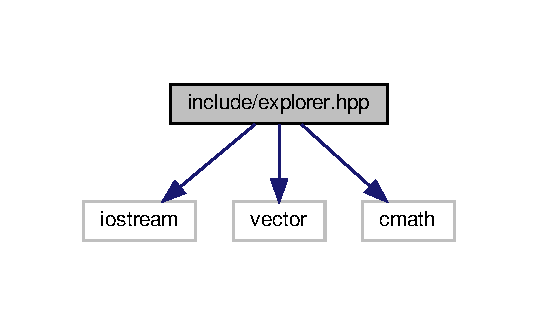
\includegraphics[width=258pt]{explorer_8hpp__incl}
\end{center}
\end{figure}
This graph shows which files directly or indirectly include this file\+:
\nopagebreak
\begin{figure}[H]
\begin{center}
\leavevmode
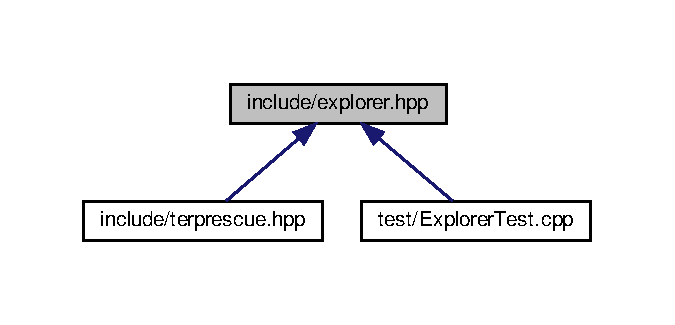
\includegraphics[width=324pt]{explorer_8hpp__dep__incl}
\end{center}
\end{figure}
\subsection*{Classes}
\begin{DoxyCompactItemize}
\item 
class \hyperlink{classExplorer}{Explorer}
\begin{DoxyCompactList}\small\item\em This class contains methods to help the robot navigate and explore the environment. \end{DoxyCompactList}\end{DoxyCompactItemize}


\subsection{Detailed Description}
This file contains delarations for the \hyperlink{classExplorer}{Explorer} class, which contains methods to help the robot navigate and explore the environment. 

Copyright (c) 2019 Jing Liang, Kevin Dong, Zuyang Cao

\begin{DoxyDate}{Date}
12/06/2019  This project is released under the B\+S\+D-\/3-\/\+Clause License. Redistribution and use in source and binary forms, with or without modification, are permitted provided that the following conditions are met\+:
\end{DoxyDate}

\begin{DoxyEnumerate}
\item Redistributions of source code must retain the above copyright notice, this list of conditions and the following disclaimer.
\item Redistributions in binary form must reproduce the above copyright notice, this list of conditions and the following disclaimer in the documentation and/or other materials provided with the distribution.
\item Neither the name of the copyright holder nor the names of its contributors may be used to endorse or promote products derived from this software without specific prior written permission.
\end{DoxyEnumerate}

T\+H\+IS S\+O\+F\+T\+W\+A\+RE IS P\+R\+O\+V\+I\+D\+ED BY T\+HE C\+O\+P\+Y\+R\+I\+G\+HT H\+O\+L\+D\+E\+RS A\+ND C\+O\+N\+T\+R\+I\+B\+U\+T\+O\+RS \char`\"{}\+A\+S I\+S\char`\"{} A\+ND A\+NY E\+X\+P\+R\+E\+SS OR I\+M\+P\+L\+I\+ED W\+A\+R\+R\+A\+N\+T\+I\+ES, I\+N\+C\+L\+U\+D\+I\+NG, B\+UT N\+OT L\+I\+M\+I\+T\+ED TO, T\+HE I\+M\+P\+L\+I\+ED W\+A\+R\+R\+A\+N\+T\+I\+ES OF M\+E\+R\+C\+H\+A\+N\+T\+A\+B\+I\+L\+I\+TY A\+ND F\+I\+T\+N\+E\+SS F\+OR A P\+A\+R\+T\+I\+C\+U\+L\+AR P\+U\+R\+P\+O\+SE A\+RE D\+I\+S\+C\+L\+A\+I\+M\+ED. IN NO E\+V\+E\+NT S\+H\+A\+LL T\+HE C\+O\+P\+Y\+R\+I\+G\+HT H\+O\+L\+D\+ER OR C\+O\+N\+T\+R\+I\+B\+U\+T\+O\+RS BE L\+I\+A\+B\+LE F\+OR A\+NY D\+I\+R\+E\+CT, I\+N\+D\+I\+R\+E\+CT, I\+N\+C\+I\+D\+E\+N\+T\+AL, S\+P\+E\+C\+I\+AL, E\+X\+E\+M\+P\+L\+A\+RY, OR C\+O\+N\+S\+E\+Q\+U\+E\+N\+T\+I\+AL D\+A\+M\+A\+G\+ES (I\+N\+C\+L\+U\+D\+I\+NG, B\+UT N\+OT L\+I\+M\+I\+T\+ED TO, P\+R\+O\+C\+U\+R\+E\+M\+E\+NT OF S\+U\+B\+S\+T\+I\+T\+U\+TE G\+O\+O\+DS OR S\+E\+R\+V\+I\+C\+ES; L\+O\+SS OF U\+SE, D\+A\+TA, OR P\+R\+O\+F\+I\+TS; OR B\+U\+S\+I\+N\+E\+SS I\+N\+T\+E\+R\+R\+U\+P\+T\+I\+ON) H\+O\+W\+E\+V\+ER C\+A\+U\+S\+ED A\+ND ON A\+NY T\+H\+E\+O\+RY OF L\+I\+A\+B\+I\+L\+I\+TY, W\+H\+E\+T\+H\+ER IN C\+O\+N\+T\+R\+A\+CT, S\+T\+R\+I\+CT L\+I\+A\+B\+I\+L\+I\+TY, OR T\+O\+RT (I\+N\+C\+L\+U\+D\+I\+NG N\+E\+G\+L\+I\+G\+E\+N\+CE OR O\+T\+H\+E\+R\+W\+I\+SE) A\+R\+I\+S\+I\+NG IN A\+NY W\+AY O\+UT OF T\+HE U\+SE OF T\+H\+IS S\+O\+F\+T\+W\+A\+RE, E\+V\+EN IF A\+D\+V\+I\+S\+ED OF T\+HE P\+O\+S\+S\+I\+B\+I\+L\+I\+TY OF S\+U\+CH D\+A\+M\+A\+GE. 
\hypertarget{localizer_8hpp}{}\section{include/localizer.hpp File Reference}
\label{localizer_8hpp}\index{include/localizer.\+hpp@{include/localizer.\+hpp}}


This class defined class of localizer which is the class calculating tags positions And also recognize tag ID  This project is released under the B\+S\+D-\/3-\/\+Clause License. Redistribution and use in source and binary forms, with or without modification, are permitted provided that the following conditions are met\+:  


{\ttfamily \#include $<$ros/ros.\+h$>$}\newline
{\ttfamily \#include $<$geometry\+\_\+msgs/\+Pose.\+h$>$}\newline
{\ttfamily \#include $<$ar\+\_\+track\+\_\+alvar\+\_\+msgs/\+Alvar\+Marker.\+h$>$}\newline
{\ttfamily \#include $<$geometry\+\_\+msgs/\+Pose\+Stamped.\+h$>$}\newline
{\ttfamily \#include $<$tf2/\+Linear\+Math/\+Quaternion.\+h$>$}\newline
{\ttfamily \#include $<$tf2/\+Linear\+Math/\+Transform.\+h$>$}\newline
{\ttfamily \#include $<$tf2\+\_\+geometry\+\_\+msgs/tf2\+\_\+geometry\+\_\+msgs.\+h$>$}\newline
{\ttfamily \#include $<$nav\+\_\+msgs/\+Odometry.\+h$>$}\newline
{\ttfamily \#include $<$vector$>$}\newline
Include dependency graph for localizer.\+hpp\+:
\nopagebreak
\begin{figure}[H]
\begin{center}
\leavevmode
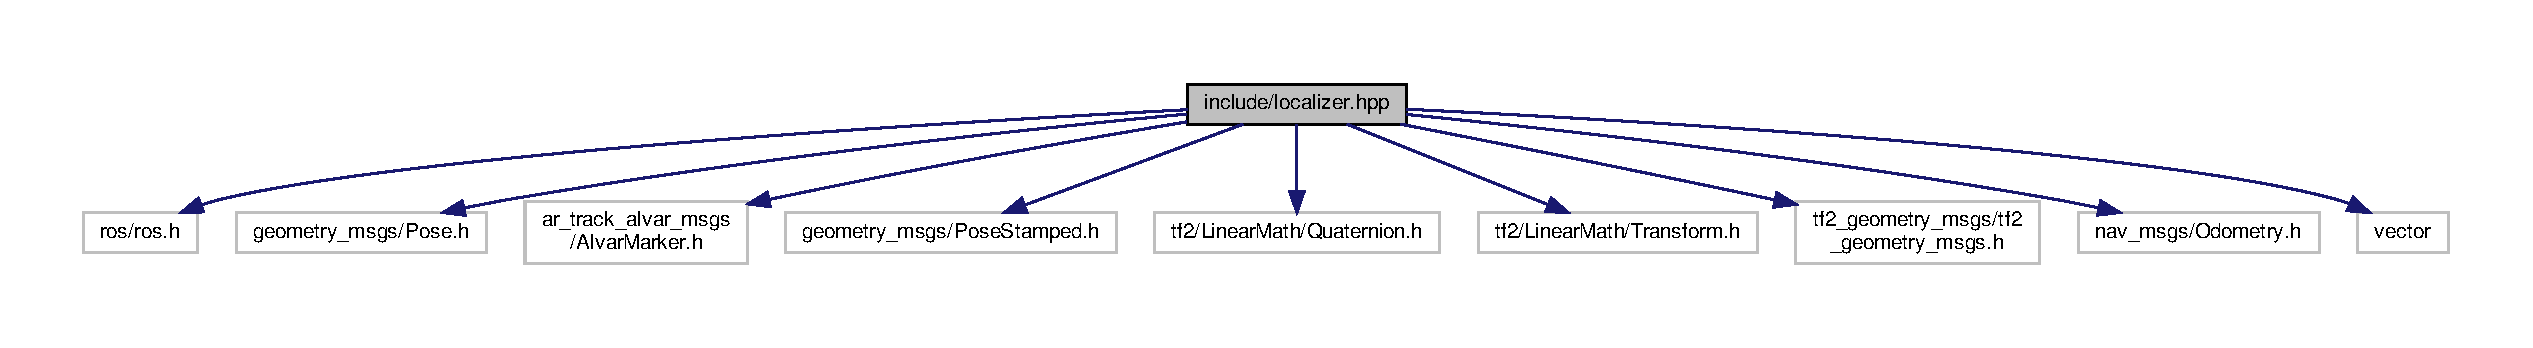
\includegraphics[width=350pt]{localizer_8hpp__incl}
\end{center}
\end{figure}
This graph shows which files directly or indirectly include this file\+:
\nopagebreak
\begin{figure}[H]
\begin{center}
\leavevmode
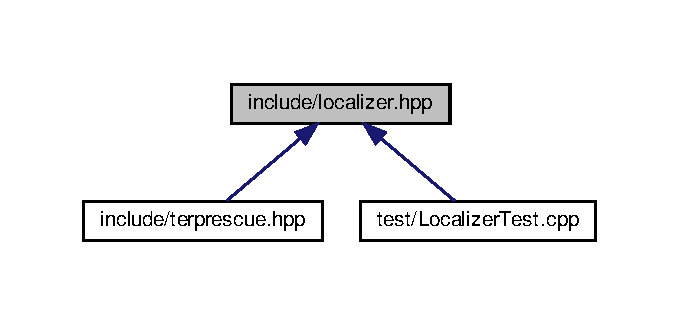
\includegraphics[width=326pt]{localizer_8hpp__dep__incl}
\end{center}
\end{figure}
\subsection*{Classes}
\begin{DoxyCompactItemize}
\item 
class \hyperlink{classLocalizer}{Localizer}
\begin{DoxyCompactList}\small\item\em The class has can use input data of lidar, camera and also robot\textquotesingle{}s frame to recognize tags and get tags\textquotesingle{} location and ID. \end{DoxyCompactList}\end{DoxyCompactItemize}


\subsection{Detailed Description}
This class defined class of localizer which is the class calculating tags positions And also recognize tag ID  This project is released under the B\+S\+D-\/3-\/\+Clause License. Redistribution and use in source and binary forms, with or without modification, are permitted provided that the following conditions are met\+: 

Copyright (c) 2019 Jing Liang, Kevin Dong, Zuyang Cao

\begin{DoxyDate}{Date}
11/23/2019
\begin{DoxyEnumerate}
\item Redistributions of source code must retain the above copyright notice, this list of conditions and the following disclaimer.
\item Redistributions in binary form must reproduce the above copyright notice, this list of conditions and the following disclaimer in the documentation and/or other materials provided with the distribution.
\item Neither the name of the copyright holder nor the names of its contributors may be used to endorse or promote products derived from this software without specific prior written permission.
\end{DoxyEnumerate}
\end{DoxyDate}
T\+H\+IS S\+O\+F\+T\+W\+A\+RE IS P\+R\+O\+V\+I\+D\+ED BY T\+HE C\+O\+P\+Y\+R\+I\+G\+HT H\+O\+L\+D\+E\+RS A\+ND C\+O\+N\+T\+R\+I\+B\+U\+T\+O\+RS \char`\"{}\+A\+S I\+S\char`\"{} A\+ND A\+NY E\+X\+P\+R\+E\+SS OR I\+M\+P\+L\+I\+ED W\+A\+R\+R\+A\+N\+T\+I\+ES, I\+N\+C\+L\+U\+D\+I\+NG, B\+UT N\+OT L\+I\+M\+I\+T\+ED TO, T\+HE I\+M\+P\+L\+I\+ED W\+A\+R\+R\+A\+N\+T\+I\+ES OF M\+E\+R\+C\+H\+A\+N\+T\+A\+B\+I\+L\+I\+TY A\+ND F\+I\+T\+N\+E\+SS F\+OR A P\+A\+R\+T\+I\+C\+U\+L\+AR P\+U\+R\+P\+O\+SE A\+RE D\+I\+S\+C\+L\+A\+I\+M\+ED. IN NO E\+V\+E\+NT S\+H\+A\+LL T\+HE C\+O\+P\+Y\+R\+I\+G\+HT H\+O\+L\+D\+ER OR C\+O\+N\+T\+R\+I\+B\+U\+T\+O\+RS BE L\+I\+A\+B\+LE F\+OR A\+NY D\+I\+R\+E\+CT, I\+N\+D\+I\+R\+E\+CT, I\+N\+C\+I\+D\+E\+N\+T\+AL, S\+P\+E\+C\+I\+AL, E\+X\+E\+M\+P\+L\+A\+RY, OR C\+O\+N\+S\+E\+Q\+U\+E\+N\+T\+I\+AL D\+A\+M\+A\+G\+ES (I\+N\+C\+L\+U\+D\+I\+NG, B\+UT N\+OT L\+I\+M\+I\+T\+ED TO, P\+R\+O\+C\+U\+R\+E\+M\+E\+NT OF S\+U\+B\+S\+T\+I\+T\+U\+TE G\+O\+O\+DS OR S\+E\+R\+V\+I\+C\+ES; L\+O\+SS OF U\+SE, D\+A\+TA, OR P\+R\+O\+F\+I\+TS; OR B\+U\+S\+I\+N\+E\+SS I\+N\+T\+E\+R\+R\+U\+P\+T\+I\+ON) H\+O\+W\+E\+V\+ER C\+A\+U\+S\+ED A\+ND ON A\+NY T\+H\+E\+O\+RY OF L\+I\+A\+B\+I\+L\+I\+TY, W\+H\+E\+T\+H\+ER IN C\+O\+N\+T\+R\+A\+CT, S\+T\+R\+I\+CT L\+I\+A\+B\+I\+L\+I\+TY, OR T\+O\+RT (I\+N\+C\+L\+U\+D\+I\+NG N\+E\+G\+L\+I\+G\+E\+N\+CE OR O\+T\+H\+E\+R\+W\+I\+SE) A\+R\+I\+S\+I\+NG IN A\+NY W\+AY O\+UT OF T\+HE U\+SE OF T\+H\+IS S\+O\+F\+T\+W\+A\+RE, E\+V\+EN IF A\+D\+V\+I\+S\+ED OF T\+HE P\+O\+S\+S\+I\+B\+I\+L\+I\+TY OF S\+U\+CH D\+A\+M\+A\+GE. 
\hypertarget{terprescue_8hpp}{}\section{include/terprescue.hpp File Reference}
\label{terprescue_8hpp}\index{include/terprescue.\+hpp@{include/terprescue.\+hpp}}


This class defined class of \hyperlink{classTerpRescue}{Terp\+Rescue} which is the main class of this project The class has functions to subscribe all sensor data and also calculate tag location and display map in rviz.  This project is released under the B\+S\+D-\/3-\/\+Clause License. Redistribution and use in source and binary forms, with or without modification, are permitted provided that the following conditions are met\+:  


{\ttfamily \#include $<$ros/ros.\+h$>$}\newline
{\ttfamily \#include $<$sensor\+\_\+msgs/\+Laser\+Scan.\+h$>$}\newline
{\ttfamily \#include $<$geometry\+\_\+msgs/\+Pose.\+h$>$}\newline
{\ttfamily \#include $<$geometry\+\_\+msgs/\+Twist.\+h$>$}\newline
{\ttfamily \#include $<$sensor\+\_\+msgs/\+Image.\+h$>$}\newline
{\ttfamily \#include $<$nav\+\_\+msgs/\+Odometry.\+h$>$}\newline
{\ttfamily \#include $<$nav\+\_\+msgs/\+Occupancy\+Grid.\+h$>$}\newline
{\ttfamily \#include $<$gazebo\+\_\+msgs/\+Model\+States.\+h$>$}\newline
{\ttfamily \#include $<$ar\+\_\+track\+\_\+alvar\+\_\+msgs/\+Alvar\+Marker.\+h$>$}\newline
{\ttfamily \#include $<$ar\+\_\+track\+\_\+alvar\+\_\+msgs/\+Alvar\+Markers.\+h$>$}\newline
{\ttfamily \#include $<$geometry\+\_\+msgs/\+Pose\+Stamped.\+h$>$}\newline
{\ttfamily \#include $<$visualization\+\_\+msgs/\+Marker.\+h$>$}\newline
{\ttfamily \#include $<$visualization\+\_\+msgs/\+Marker\+Array.\+h$>$}\newline
{\ttfamily \#include $<$vector$>$}\newline
{\ttfamily \#include $<$string$>$}\newline
{\ttfamily \#include $<$cmath$>$}\newline
{\ttfamily \#include $<$ctime$>$}\newline
{\ttfamily \#include $<$localizer.\+hpp$>$}\newline
{\ttfamily \#include $<$explorer.\+hpp$>$}\newline
Include dependency graph for terprescue.\+hpp\+:
\nopagebreak
\begin{figure}[H]
\begin{center}
\leavevmode
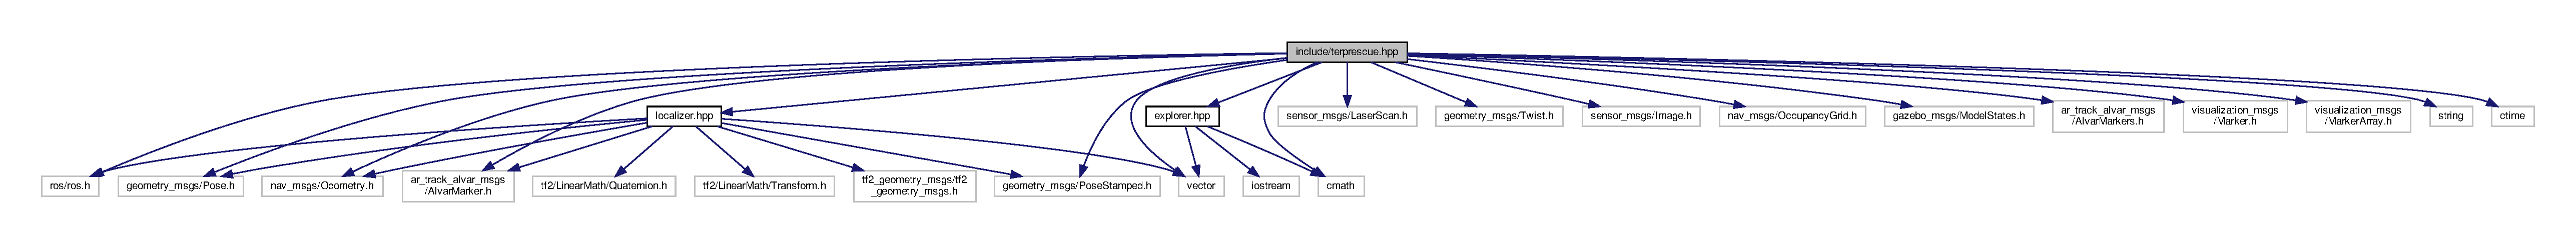
\includegraphics[width=350pt]{terprescue_8hpp__incl}
\end{center}
\end{figure}
\subsection*{Classes}
\begin{DoxyCompactItemize}
\item 
class \hyperlink{classTerpRescue}{Terp\+Rescue}
\begin{DoxyCompactList}\small\item\em The class has functions to subscribe all sensor data and also calculate tag location and display map in R\+Viz. \end{DoxyCompactList}\end{DoxyCompactItemize}


\subsection{Detailed Description}
This class defined class of \hyperlink{classTerpRescue}{Terp\+Rescue} which is the main class of this project The class has functions to subscribe all sensor data and also calculate tag location and display map in rviz.  This project is released under the B\+S\+D-\/3-\/\+Clause License. Redistribution and use in source and binary forms, with or without modification, are permitted provided that the following conditions are met\+: 

Copyright (c) 2019 Jing Liang, Kevin Dong, Zuyang Cao

\begin{DoxyDate}{Date}
11/23/2019
\begin{DoxyEnumerate}
\item Redistributions of source code must retain the above copyright notice, this list of conditions and the following disclaimer.
\item Redistributions in binary form must reproduce the above copyright notice, this list of conditions and the following disclaimer in the documentation and/or other materials provided with the distribution.
\item Neither the name of the copyright holder nor the names of its contributors may be used to endorse or promote products derived from this software without specific prior written permission.
\end{DoxyEnumerate}
\end{DoxyDate}
T\+H\+IS S\+O\+F\+T\+W\+A\+RE IS P\+R\+O\+V\+I\+D\+ED BY T\+HE C\+O\+P\+Y\+R\+I\+G\+HT H\+O\+L\+D\+E\+RS A\+ND C\+O\+N\+T\+R\+I\+B\+U\+T\+O\+RS \char`\"{}\+A\+S I\+S\char`\"{} A\+ND A\+NY E\+X\+P\+R\+E\+SS OR I\+M\+P\+L\+I\+ED W\+A\+R\+R\+A\+N\+T\+I\+ES, I\+N\+C\+L\+U\+D\+I\+NG, B\+UT N\+OT L\+I\+M\+I\+T\+ED TO, T\+HE I\+M\+P\+L\+I\+ED W\+A\+R\+R\+A\+N\+T\+I\+ES OF M\+E\+R\+C\+H\+A\+N\+T\+A\+B\+I\+L\+I\+TY A\+ND F\+I\+T\+N\+E\+SS F\+OR A P\+A\+R\+T\+I\+C\+U\+L\+AR P\+U\+R\+P\+O\+SE A\+RE D\+I\+S\+C\+L\+A\+I\+M\+ED. IN NO E\+V\+E\+NT S\+H\+A\+LL T\+HE C\+O\+P\+Y\+R\+I\+G\+HT H\+O\+L\+D\+ER OR C\+O\+N\+T\+R\+I\+B\+U\+T\+O\+RS BE L\+I\+A\+B\+LE F\+OR A\+NY D\+I\+R\+E\+CT, I\+N\+D\+I\+R\+E\+CT, I\+N\+C\+I\+D\+E\+N\+T\+AL, S\+P\+E\+C\+I\+AL, E\+X\+E\+M\+P\+L\+A\+RY, OR C\+O\+N\+S\+E\+Q\+U\+E\+N\+T\+I\+AL D\+A\+M\+A\+G\+ES (I\+N\+C\+L\+U\+D\+I\+NG, B\+UT N\+OT L\+I\+M\+I\+T\+ED TO, P\+R\+O\+C\+U\+R\+E\+M\+E\+NT OF S\+U\+B\+S\+T\+I\+T\+U\+TE G\+O\+O\+DS OR S\+E\+R\+V\+I\+C\+ES; L\+O\+SS OF U\+SE, D\+A\+TA, OR P\+R\+O\+F\+I\+TS; OR B\+U\+S\+I\+N\+E\+SS I\+N\+T\+E\+R\+R\+U\+P\+T\+I\+ON) H\+O\+W\+E\+V\+ER C\+A\+U\+S\+ED A\+ND ON A\+NY T\+H\+E\+O\+RY OF L\+I\+A\+B\+I\+L\+I\+TY, W\+H\+E\+T\+H\+ER IN C\+O\+N\+T\+R\+A\+CT, S\+T\+R\+I\+CT L\+I\+A\+B\+I\+L\+I\+TY, OR T\+O\+RT (I\+N\+C\+L\+U\+D\+I\+NG N\+E\+G\+L\+I\+G\+E\+N\+CE OR O\+T\+H\+E\+R\+W\+I\+SE) A\+R\+I\+S\+I\+NG IN A\+NY W\+AY O\+UT OF T\+HE U\+SE OF T\+H\+IS S\+O\+F\+T\+W\+A\+RE, E\+V\+EN IF A\+D\+V\+I\+S\+ED OF T\+HE P\+O\+S\+S\+I\+B\+I\+L\+I\+TY OF S\+U\+CH D\+A\+M\+A\+GE. 
\hypertarget{ExplorerTest_8cpp}{}\section{test/\+Explorer\+Test.cpp File Reference}
\label{ExplorerTest_8cpp}\index{test/\+Explorer\+Test.\+cpp@{test/\+Explorer\+Test.\+cpp}}


\hyperlink{classExplorer}{Explorer} class test file  B\+SD 3-\/\+Clause L\+I\+C\+E\+N\+SE.  


{\ttfamily \#include $<$gtest/gtest.\+h$>$}\newline
{\ttfamily \#include $<$vector$>$}\newline
{\ttfamily \#include $<$explorer.\+hpp$>$}\newline
Include dependency graph for Explorer\+Test.\+cpp\+:
\nopagebreak
\begin{figure}[H]
\begin{center}
\leavevmode
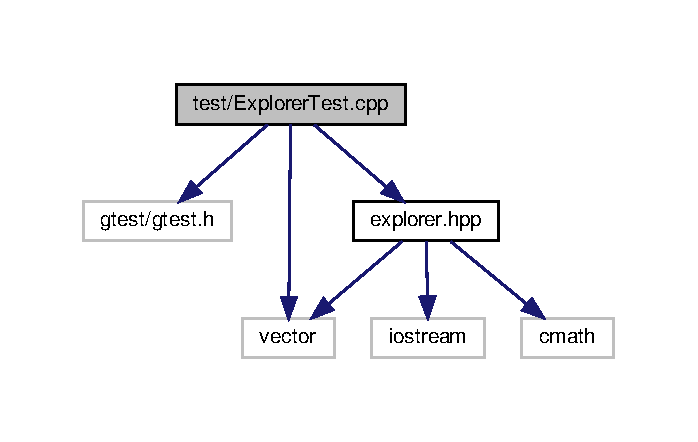
\includegraphics[width=335pt]{ExplorerTest_8cpp__incl}
\end{center}
\end{figure}
\subsection*{Functions}
\begin{DoxyCompactItemize}
\item 
\mbox{\Hypertarget{ExplorerTest_8cpp_a58a6e3a3aede9cf72a105a74d3ad824f}\label{ExplorerTest_8cpp_a58a6e3a3aede9cf72a105a74d3ad824f}} 
{\bfseries T\+E\+ST} (\hyperlink{classExplorer}{Explorer}, detect\+Object\+Test)
\item 
\mbox{\Hypertarget{ExplorerTest_8cpp_a21b28cb9e6373cc779a8027cc1f10e23}\label{ExplorerTest_8cpp_a21b28cb9e6373cc779a8027cc1f10e23}} 
{\bfseries T\+E\+ST} (\hyperlink{classExplorer}{Explorer}, update\+Lidar\+Costs\+Test)
\end{DoxyCompactItemize}


\subsection{Detailed Description}
\hyperlink{classExplorer}{Explorer} class test file  B\+SD 3-\/\+Clause L\+I\+C\+E\+N\+SE. 

Copyright (c) 2019 Jing Liang, Kevin Dong, Zuyang Cao

Copyright (c) 2018, Zuyang Cao All rights reserved.

Redistribution and use in source and binary forms, with or without modification, are permitted provided that the following conditions are met\+:


\begin{DoxyEnumerate}
\item Redistributions of source code must retain the above copyright notice, this list of conditions and the following disclaimer.
\item Redistributions in binary form must reproduce the above copyright notice, this list of conditions and the following disclaimer in the documentation and/or other materials provided with the distribution.
\item Neither the name of the copyright holder nor the names of its contributors may be used to endorse or promote products derived from this software without specific prior written permission.
\end{DoxyEnumerate}

T\+H\+IS S\+O\+F\+T\+W\+A\+RE IS P\+R\+O\+V\+I\+D\+ED BY T\+HE C\+O\+P\+Y\+R\+I\+G\+HT H\+O\+L\+D\+E\+RS A\+ND C\+O\+N\+T\+R\+I\+B\+U\+T\+O\+RS \char`\"{}\+A\+S
\+I\+S\char`\"{} A\+ND A\+NY E\+X\+P\+R\+E\+SS OR I\+M\+P\+L\+I\+ED W\+A\+R\+R\+A\+N\+T\+I\+ES, I\+N\+C\+L\+U\+D\+I\+NG, B\+UT N\+OT L\+I\+M\+I\+T\+ED TO, T\+HE I\+M\+P\+L\+I\+ED W\+A\+R\+R\+A\+N\+T\+I\+ES OF M\+E\+R\+C\+H\+A\+N\+T\+A\+B\+I\+L\+I\+TY A\+ND F\+I\+T\+N\+E\+SS F\+OR A P\+A\+R\+T\+I\+C\+U\+L\+AR P\+U\+R\+P\+O\+SE A\+RE D\+I\+S\+C\+L\+A\+I\+M\+ED. IN NO E\+V\+E\+NT S\+H\+A\+LL T\+HE C\+O\+P\+Y\+R\+I\+G\+HT H\+O\+L\+D\+ER OR C\+O\+N\+T\+R\+I\+B\+U\+T\+O\+RS BE L\+I\+A\+B\+LE F\+OR A\+NY D\+I\+R\+E\+CT, I\+N\+D\+I\+R\+E\+CT, I\+N\+C\+I\+D\+E\+N\+T\+AL, S\+P\+E\+C\+I\+AL, E\+X\+E\+M\+P\+L\+A\+RY, OR C\+O\+N\+S\+E\+Q\+U\+E\+N\+T\+I\+AL D\+A\+M\+A\+G\+ES (I\+N\+C\+L\+U\+D\+I\+NG, B\+UT N\+OT L\+I\+M\+I\+T\+ED TO, P\+R\+O\+C\+U\+R\+E\+M\+E\+NT OF S\+U\+B\+S\+T\+I\+T\+U\+TE G\+O\+O\+DS OR S\+E\+R\+V\+I\+C\+ES; L\+O\+SS OF U\+SE, D\+A\+TA, OR P\+R\+O\+F\+I\+TS; OR B\+U\+S\+I\+N\+E\+SS I\+N\+T\+E\+R\+R\+U\+P\+T\+I\+ON) H\+O\+W\+E\+V\+ER C\+A\+U\+S\+ED A\+ND ON A\+NY T\+H\+E\+O\+RY OF L\+I\+A\+B\+I\+L\+I\+TY, W\+H\+E\+T\+H\+ER IN C\+O\+N\+T\+R\+A\+CT, S\+T\+R\+I\+CT L\+I\+A\+B\+I\+L\+I\+TY, OR T\+O\+RT (I\+N\+C\+L\+U\+D\+I\+NG N\+E\+G\+L\+I\+G\+E\+N\+CE OR O\+T\+H\+E\+R\+W\+I\+SE) A\+R\+I\+S\+I\+NG IN A\+NY W\+AY O\+UT OF T\+HE U\+SE OF T\+H\+IS S\+O\+F\+T\+W\+A\+RE, E\+V\+EN IF A\+D\+V\+I\+S\+ED OF T\+HE P\+O\+S\+S\+I\+B\+I\+L\+I\+TY OF S\+U\+CH D\+A\+M\+A\+GE. 
\hypertarget{LocalizerTest_8cpp}{}\section{test/\+Localizer\+Test.cpp File Reference}
\label{LocalizerTest_8cpp}\index{test/\+Localizer\+Test.\+cpp@{test/\+Localizer\+Test.\+cpp}}


\hyperlink{classLocalizer}{Localizer} class test file  B\+SD 3-\/\+Clause L\+I\+C\+E\+N\+SE.  


{\ttfamily \#include $<$gtest/gtest.\+h$>$}\newline
{\ttfamily \#include $<$ros/package.\+h$>$}\newline
{\ttfamily \#include $<$ros/ros.\+h$>$}\newline
{\ttfamily \#include $<$vector$>$}\newline
{\ttfamily \#include $<$localizer.\+hpp$>$}\newline
Include dependency graph for Localizer\+Test.\+cpp\+:
\nopagebreak
\begin{figure}[H]
\begin{center}
\leavevmode
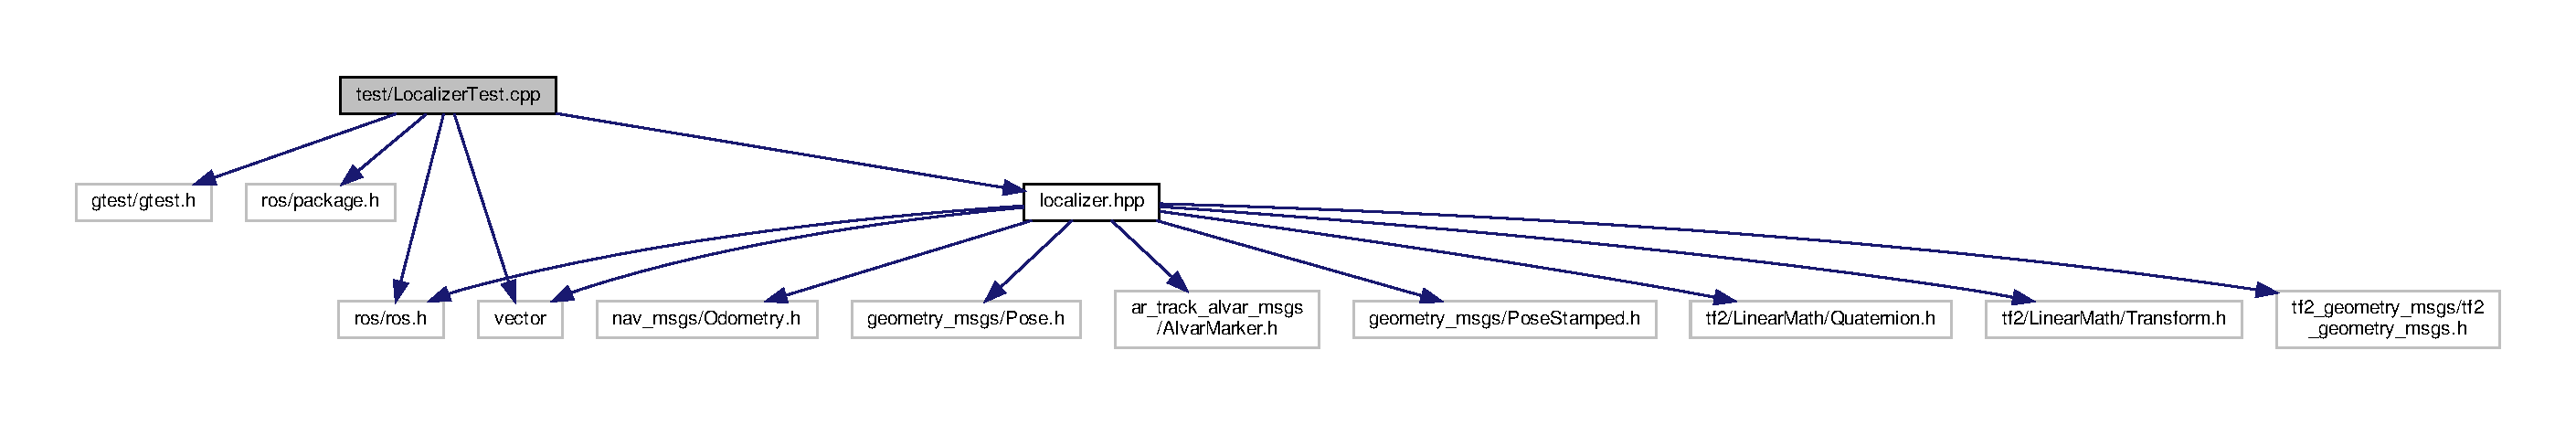
\includegraphics[width=350pt]{LocalizerTest_8cpp__incl}
\end{center}
\end{figure}
\subsection*{Functions}
\begin{DoxyCompactItemize}
\item 
\hyperlink{LocalizerTest_8cpp_a94e15e660860bc71531024e39f3a186e}{T\+E\+ST} (\hyperlink{classLocalizer}{Localizer}, Dummy\+Test)
\begin{DoxyCompactList}\small\item\em Dummy test. \end{DoxyCompactList}\item 
\mbox{\Hypertarget{LocalizerTest_8cpp_a75a395261c6e86e7d2d33046f23cf2f5}\label{LocalizerTest_8cpp_a75a395261c6e86e7d2d33046f23cf2f5}} 
{\bfseries T\+E\+ST} (\hyperlink{classLocalizer}{Localizer}, recognize\+Tag\+No\+Marker\+Test)
\item 
\mbox{\Hypertarget{LocalizerTest_8cpp_a5794ab399602766d6b8958e333aae32e}\label{LocalizerTest_8cpp_a5794ab399602766d6b8958e333aae32e}} 
{\bfseries T\+E\+ST} (\hyperlink{classLocalizer}{Localizer}, recognize\+Tag\+Zero\+Marker\+Test)
\item 
\mbox{\Hypertarget{LocalizerTest_8cpp_a8155101884a9b7219675b1fadcbb113f}\label{LocalizerTest_8cpp_a8155101884a9b7219675b1fadcbb113f}} 
{\bfseries T\+E\+ST} (\hyperlink{classLocalizer}{Localizer}, recognize\+Tag\+Nan\+Marker\+Test)
\item 
\mbox{\Hypertarget{LocalizerTest_8cpp_a1b801888b940f4c781bd52b0f44f5c34}\label{LocalizerTest_8cpp_a1b801888b940f4c781bd52b0f44f5c34}} 
{\bfseries T\+E\+ST} (\hyperlink{classLocalizer}{Localizer}, locate\+Tag\+No\+Marker\+Test)
\item 
\mbox{\Hypertarget{LocalizerTest_8cpp_a20b9a8a47fa8438ce76c06ea6476af26}\label{LocalizerTest_8cpp_a20b9a8a47fa8438ce76c06ea6476af26}} 
{\bfseries T\+E\+ST} (\hyperlink{classLocalizer}{Localizer}, locate\+Tag\+One\+Marker\+Test)
\item 
\mbox{\Hypertarget{LocalizerTest_8cpp_addd2ffd937a3268ad282927d79724457}\label{LocalizerTest_8cpp_addd2ffd937a3268ad282927d79724457}} 
{\bfseries T\+E\+ST} (\hyperlink{classLocalizer}{Localizer}, transformation\+Tag\+Position\+No\+Marker\+Test)
\item 
\mbox{\Hypertarget{LocalizerTest_8cpp_a43d537eb08c566516e1a89e5a77e0420}\label{LocalizerTest_8cpp_a43d537eb08c566516e1a89e5a77e0420}} 
{\bfseries T\+E\+ST} (\hyperlink{classLocalizer}{Localizer}, transformation\+Tag\+Position\+One\+Marker\+Test)
\end{DoxyCompactItemize}


\subsection{Detailed Description}
\hyperlink{classLocalizer}{Localizer} class test file  B\+SD 3-\/\+Clause L\+I\+C\+E\+N\+SE. 

Copyright (c) 2019 Jing Liang, Kevin Dong, Zuyang Cao

Copyright (c) 2018, Zuyang Cao All rights reserved.

Redistribution and use in source and binary forms, with or without modification, are permitted provided that the following conditions are met\+:


\begin{DoxyEnumerate}
\item Redistributions of source code must retain the above copyright notice, this list of conditions and the following disclaimer.
\item Redistributions in binary form must reproduce the above copyright notice, this list of conditions and the following disclaimer in the documentation and/or other materials provided with the distribution.
\item Neither the name of the copyright holder nor the names of its contributors may be used to endorse or promote products derived from this software without specific prior written permission.
\end{DoxyEnumerate}

T\+H\+IS S\+O\+F\+T\+W\+A\+RE IS P\+R\+O\+V\+I\+D\+ED BY T\+HE C\+O\+P\+Y\+R\+I\+G\+HT H\+O\+L\+D\+E\+RS A\+ND C\+O\+N\+T\+R\+I\+B\+U\+T\+O\+RS \char`\"{}\+A\+S
\+I\+S\char`\"{} A\+ND A\+NY E\+X\+P\+R\+E\+SS OR I\+M\+P\+L\+I\+ED W\+A\+R\+R\+A\+N\+T\+I\+ES, I\+N\+C\+L\+U\+D\+I\+NG, B\+UT N\+OT L\+I\+M\+I\+T\+ED TO, T\+HE I\+M\+P\+L\+I\+ED W\+A\+R\+R\+A\+N\+T\+I\+ES OF M\+E\+R\+C\+H\+A\+N\+T\+A\+B\+I\+L\+I\+TY A\+ND F\+I\+T\+N\+E\+SS F\+OR A P\+A\+R\+T\+I\+C\+U\+L\+AR P\+U\+R\+P\+O\+SE A\+RE D\+I\+S\+C\+L\+A\+I\+M\+ED. IN NO E\+V\+E\+NT S\+H\+A\+LL T\+HE C\+O\+P\+Y\+R\+I\+G\+HT H\+O\+L\+D\+ER OR C\+O\+N\+T\+R\+I\+B\+U\+T\+O\+RS BE L\+I\+A\+B\+LE F\+OR A\+NY D\+I\+R\+E\+CT, I\+N\+D\+I\+R\+E\+CT, I\+N\+C\+I\+D\+E\+N\+T\+AL, S\+P\+E\+C\+I\+AL, E\+X\+E\+M\+P\+L\+A\+RY, OR C\+O\+N\+S\+E\+Q\+U\+E\+N\+T\+I\+AL D\+A\+M\+A\+G\+ES (I\+N\+C\+L\+U\+D\+I\+NG, B\+UT N\+OT L\+I\+M\+I\+T\+ED TO, P\+R\+O\+C\+U\+R\+E\+M\+E\+NT OF S\+U\+B\+S\+T\+I\+T\+U\+TE G\+O\+O\+DS OR S\+E\+R\+V\+I\+C\+ES; L\+O\+SS OF U\+SE, D\+A\+TA, OR P\+R\+O\+F\+I\+TS; OR B\+U\+S\+I\+N\+E\+SS I\+N\+T\+E\+R\+R\+U\+P\+T\+I\+ON) H\+O\+W\+E\+V\+ER C\+A\+U\+S\+ED A\+ND ON A\+NY T\+H\+E\+O\+RY OF L\+I\+A\+B\+I\+L\+I\+TY, W\+H\+E\+T\+H\+ER IN C\+O\+N\+T\+R\+A\+CT, S\+T\+R\+I\+CT L\+I\+A\+B\+I\+L\+I\+TY, OR T\+O\+RT (I\+N\+C\+L\+U\+D\+I\+NG N\+E\+G\+L\+I\+G\+E\+N\+CE OR O\+T\+H\+E\+R\+W\+I\+SE) A\+R\+I\+S\+I\+NG IN A\+NY W\+AY O\+UT OF T\+HE U\+SE OF T\+H\+IS S\+O\+F\+T\+W\+A\+RE, E\+V\+EN IF A\+D\+V\+I\+S\+ED OF T\+HE P\+O\+S\+S\+I\+B\+I\+L\+I\+TY OF S\+U\+CH D\+A\+M\+A\+GE. 

\subsection{Function Documentation}
\mbox{\Hypertarget{LocalizerTest_8cpp_a94e15e660860bc71531024e39f3a186e}\label{LocalizerTest_8cpp_a94e15e660860bc71531024e39f3a186e}} 
\index{Localizer\+Test.\+cpp@{Localizer\+Test.\+cpp}!T\+E\+ST@{T\+E\+ST}}
\index{T\+E\+ST@{T\+E\+ST}!Localizer\+Test.\+cpp@{Localizer\+Test.\+cpp}}
\subsubsection{\texorpdfstring{T\+E\+S\+T()}{TEST()}}
{\footnotesize\ttfamily T\+E\+ST (\begin{DoxyParamCaption}\item[{\hyperlink{classLocalizer}{Localizer}}]{,  }\item[{Dummy\+Test}]{ }\end{DoxyParamCaption})}



Dummy test. 


\begin{DoxyParams}[1]{Parameters}
\mbox{\tt in}  & {\em T\+E\+S\+T\+Suite} & \\
\hline
\mbox{\tt in}  & {\em test\+Service} & \\
\hline
\end{DoxyParams}
\begin{DoxyReturn}{Returns}
none 
\end{DoxyReturn}

\hypertarget{main_8cpp}{}\section{test/main.cpp File Reference}
\label{main_8cpp}\index{test/main.\+cpp@{test/main.\+cpp}}


gtest main file  B\+SD 3-\/\+Clause L\+I\+C\+E\+N\+SE  


{\ttfamily \#include $<$gtest/gtest.\+h$>$}\newline
{\ttfamily \#include $<$ros/ros.\+h$>$}\newline
Include dependency graph for main.\+cpp\+:
\nopagebreak
\begin{figure}[H]
\begin{center}
\leavevmode
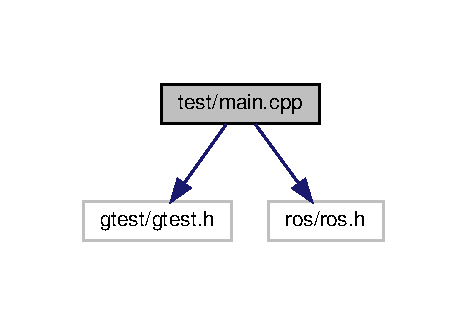
\includegraphics[width=224pt]{main_8cpp__incl}
\end{center}
\end{figure}
\subsection*{Functions}
\begin{DoxyCompactItemize}
\item 
\mbox{\Hypertarget{main_8cpp_a3c04138a5bfe5d72780bb7e82a18e627}\label{main_8cpp_a3c04138a5bfe5d72780bb7e82a18e627}} 
int {\bfseries main} (int argc, char $\ast$$\ast$argv)
\end{DoxyCompactItemize}


\subsection{Detailed Description}
gtest main file  B\+SD 3-\/\+Clause L\+I\+C\+E\+N\+SE 

Copyright (c) 2019 Jing Liang, Kevin Dong, Zuyang Cao

Copyright (c) 2018, Zuyang Cao All rights reserved.

Redistribution and use in source and binary forms, with or without modification, are permitted provided that the following conditions are met\+:


\begin{DoxyEnumerate}
\item Redistributions of source code must retain the above copyright notice, this list of conditions and the following disclaimer.
\item Redistributions in binary form must reproduce the above copyright notice, this list of conditions and the following disclaimer in the documentation and/or other materials provided with the distribution.
\item Neither the name of the copyright holder nor the names of its contributors may be used to endorse or promote products derived from this software without specific prior written permission.
\end{DoxyEnumerate}

T\+H\+IS S\+O\+F\+T\+W\+A\+RE IS P\+R\+O\+V\+I\+D\+ED BY T\+HE C\+O\+P\+Y\+R\+I\+G\+HT H\+O\+L\+D\+E\+RS A\+ND C\+O\+N\+T\+R\+I\+B\+U\+T\+O\+RS \char`\"{}\+A\+S
\+I\+S\char`\"{} A\+ND A\+NY E\+X\+P\+R\+E\+SS OR I\+M\+P\+L\+I\+ED W\+A\+R\+R\+A\+N\+T\+I\+ES, I\+N\+C\+L\+U\+D\+I\+NG, B\+UT N\+OT L\+I\+M\+I\+T\+ED TO, T\+HE I\+M\+P\+L\+I\+ED W\+A\+R\+R\+A\+N\+T\+I\+ES OF M\+E\+R\+C\+H\+A\+N\+T\+A\+B\+I\+L\+I\+TY A\+ND F\+I\+T\+N\+E\+SS F\+OR A P\+A\+R\+T\+I\+C\+U\+L\+AR P\+U\+R\+P\+O\+SE A\+RE D\+I\+S\+C\+L\+A\+I\+M\+ED. IN NO E\+V\+E\+NT S\+H\+A\+LL T\+HE C\+O\+P\+Y\+R\+I\+G\+HT H\+O\+L\+D\+ER OR C\+O\+N\+T\+R\+I\+B\+U\+T\+O\+RS BE L\+I\+A\+B\+LE F\+OR A\+NY D\+I\+R\+E\+CT, I\+N\+D\+I\+R\+E\+CT, I\+N\+C\+I\+D\+E\+N\+T\+AL, S\+P\+E\+C\+I\+AL, E\+X\+E\+M\+P\+L\+A\+RY, OR C\+O\+N\+S\+E\+Q\+U\+E\+N\+T\+I\+AL D\+A\+M\+A\+G\+ES (I\+N\+C\+L\+U\+D\+I\+NG, B\+UT N\+OT L\+I\+M\+I\+T\+ED TO, P\+R\+O\+C\+U\+R\+E\+M\+E\+NT OF S\+U\+B\+S\+T\+I\+T\+U\+TE G\+O\+O\+DS OR S\+E\+R\+V\+I\+C\+ES; L\+O\+SS OF U\+SE, D\+A\+TA, OR P\+R\+O\+F\+I\+TS; OR B\+U\+S\+I\+N\+E\+SS I\+N\+T\+E\+R\+R\+U\+P\+T\+I\+ON) H\+O\+W\+E\+V\+ER C\+A\+U\+S\+ED A\+ND ON A\+NY T\+H\+E\+O\+RY OF L\+I\+A\+B\+I\+L\+I\+TY, W\+H\+E\+T\+H\+ER IN C\+O\+N\+T\+R\+A\+CT, S\+T\+R\+I\+CT L\+I\+A\+B\+I\+L\+I\+TY, OR T\+O\+RT (I\+N\+C\+L\+U\+D\+I\+NG N\+E\+G\+L\+I\+G\+E\+N\+CE OR O\+T\+H\+E\+R\+W\+I\+SE) A\+R\+I\+S\+I\+NG IN A\+NY W\+AY O\+UT OF T\+HE U\+SE OF T\+H\+IS S\+O\+F\+T\+W\+A\+RE, E\+V\+EN IF A\+D\+V\+I\+S\+ED OF T\+HE P\+O\+S\+S\+I\+B\+I\+L\+I\+TY OF S\+U\+CH D\+A\+M\+A\+GE. 
%--- End generated contents ---

% Index
\backmatter
\newpage
\phantomsection
\clearemptydoublepage
\addcontentsline{toc}{chapter}{Index}
\printindex

\end{document}
